\beginsong{Triodimali}[
    wuw={Olka (Erich Scholz)}, 
    pfiii={35}, 
    bo={42}, 
    kssiv={49}, 
    siru={35}, 
    tonspur={174}, 
    index={Bruder nun wird es Abend},
]

\beginverse
\endverse
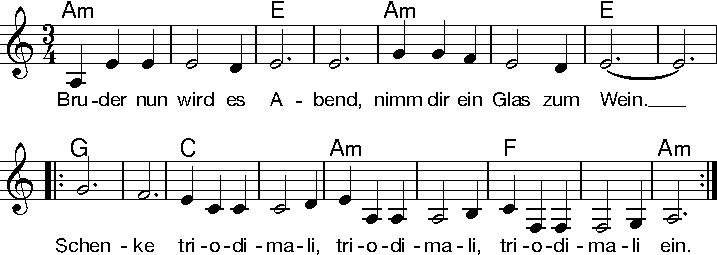
\includegraphics[draft=false, width=1\textwidth]{Noten/Lied086.pdf}	

\beginverse
\[Am]Stopf' dir die lange \[E]Pfeife, \[Am]denk' dir nicht viel da\[E]bei,
\lrep \[G]singe \[C]triodimali, \[Am]triodimali, \[F]triodimali \[Am]zwei. \rrep
\endverse

\beginverse
^Nichts will das Lied be^deuten, ^als etwas glücklich ^sein,
\lrep ^dreimal ^triodimali, ^triodimali, ^triodimlai ^drei. \rrep
\endverse

\beginverse
^Mondlampe lacht am ^Fenster, ^Schlaf klopft an die ^Tür,
\lrep ^leise ^triodimali, ^triodimali, ^triodimali ^vier. \rrep
\endverse

\beginverse
^Traumschwere Worte ^fallen, ^Stille besiegt das ^Haus,
\lrep ^trinke ^triodimali, ^triodimali, ^triodimali ^aus. \rrep
\endverse

\endsong
